\documentclass[tikz,border=10pt]{standalone}
\begin{document}

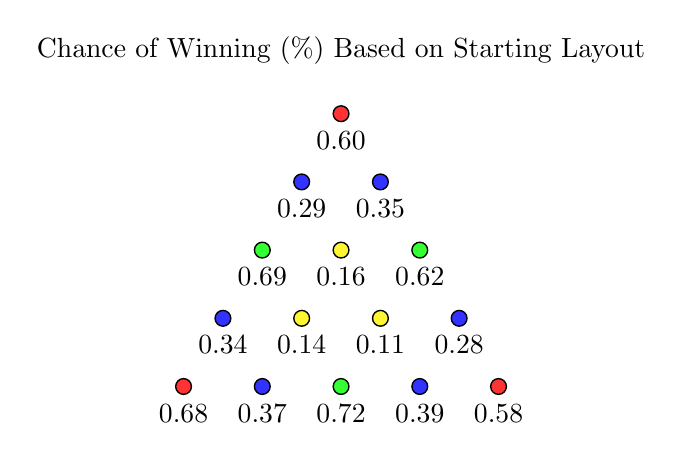
\begin{tikzpicture}

\tikzset{mycircle/.style={fill=red!80!white, draw=black, line width=0.5pt}}
\tikzset{mynode/.style={anchor=north, yshift = -0.1cm, text=black}}

\node at (0,0.8) {Chance of Winning (\%) Based on Starting Layout};

\filldraw[fill=red!80!white, draw=black, line width=0.5pt] (0,0) circle (0.1cm) node[mynode] {$0.60$};
\filldraw[fill=blue!80!white, draw=black, line width=0.5pt] (-0.5, -0.866) circle (0.1cm) node[mynode] {$0.29$};
\filldraw[fill=blue!80!white, draw=black, line width=0.5pt] (0.5,-0.866) circle (0.1cm) node[mynode] {$0.35$};
\filldraw[fill=green!80!white, draw=black, line width=0.5pt] (-1,-1.732) circle (0.1cm) node[mynode] {$0.69$};
\filldraw[fill=yellow!80!white, draw=black, line width=0.5pt] (0,-1.732) circle (0.1cm) node[mynode] {$0.16$};
\filldraw[fill=green!80!white, draw=black, line width=0.5pt] (1,-1.732) circle (0.1cm) node[mynode] {$0.62$};
\filldraw[fill=blue!80!white, draw=black, line width=0.5pt] (-1.5,-2.598) circle (0.1cm) node[mynode] {$0.34$};
\filldraw[fill=yellow!80!white, draw=black, line width=0.5pt] (-0.5,-2.598) circle (0.1cm) node[mynode] {$0.14$};
\filldraw[fill=yellow!80!white, draw=black, line width=0.5pt] (0.5,-2.598) circle (0.1cm) node[mynode] {$0.11$};
\filldraw[fill=blue!80!white, draw=black, line width=0.5pt] (1.5,-2.598) circle (0.1cm) node[mynode] {$0.28$};
\filldraw[fill=red!80!white, draw=black, line width=0.5pt] (-2,-3.464) circle (0.1cm) node[mynode] {$0.68$};
\filldraw[fill=blue!80!white, draw=black, line width=0.5pt] (-1,-3.464) circle (0.1cm) node[mynode] {$0.37$};
\filldraw[fill=green!80!white, draw=black, line width=0.5pt] (0,-3.464) circle (0.1cm) node[mynode] {$0.72$};
\filldraw[fill=blue!80!white, draw=black, line width=0.5pt] (1,-3.464) circle (0.1cm) node[mynode] {$0.39$};
\filldraw[fill=red!80!white, draw=black, line width=0.5pt] (2,-3.464) circle (0.1cm) node[mynode] {$0.58$};

\end{tikzpicture}

\end{document}